\chapter{解读计算结果}\label{ch:results}

计算结束以后，真正的分析才刚刚开始。结果图帮助我们识别趋势，数据记录说明图从哪里来，保存的工作流则规定了整个计算条件。本章介绍怎样阅读这些材料，并把它们整理成计算报告或研究记录中能够解释清楚的结论。

本章继续使用氢分子和硅两组案例。它们分别说明单点能、原子力、结构优化、能带和态密度的阅读方法。阅读自己的结果时，也可以依次问三个问题：这次计算是否完成，图中的量怎样定义，它能够支持哪一种结论。

\section{在项目中找到结果}

\subsection{结果保存在哪里}

点击左侧栏的 \ui{项目浏览器}，展开 \ui{Results}，其中的 \ui{Datasets} 保存数据集，\ui{Plots} 保存图形。数据集保存一次运行产生的计算信息，图形以便于阅读的形式呈现其中一部分。能带、DOS 和收敛图都属于图形结果，但它们表示的量不同。

双击当前版本生成的图形可以再次查看。若同一文档已经打开，应用会转到该文档。跨版本打开旧项目时，图形对象可能无法恢复；随书硅项目的保存数值仍可按后文方法重新绘图。比较多次计算时，先阅读图形名称和对应的运行记录，确认当前查看的是哪一组条件。结果仍然留在项目中，并不表示它自动跟随最近修改的节点更新。

例如，把 Ecut 从 $20$ 改为 $30$ Ha 后，原先的收敛图依然表示 $20$ Ha 的那次计算。只有重新运行并生成新的结果，才能比较两个截断能。建议在每次试算后立即给图形写一个清楚的名称，避免积累许多难以区分的默认名称。

\subsection{先读记录，再读图形}

一张图可以很快显示问题，也可能掩盖条件不一致。阅读前先确认结构、泛函、赝势、截断能和采样方式，尤其是在项目中同时存在多个结构时。对于优化计算，还应区分初始构型和最终构型。

计算报告中不必逐行抄写日志，但应保留原始记录。正式图注写出主要条件，附录或配套文件保存完整输入。这样既保持正文流畅，也使重要数字能够被复查。

\section{读取数据集}\label{sec:read-dataset}

在\ui{Results → Datasets}中选择一次运行记录，在信息浏览器核对名称、时间和说明。数据集标签通常以\ui{Run}开头，后接运行时的工作流名称。多个记录的显示名称相近时，应结合输入条件辨认，而不只看列表中的先后位置。当前信息浏览器不展开这些计算数据集的全部数值，原始内容需要在完整MATLAB\regmark{}或相应命令工作空间中进一步读取。

下面列出导出数据集后常见的数据名称，帮助把数组与产生它的任务对应起来。需要读取原始数组时，可按下一节将所选数据集导出到工作空间。

\begin{table}[htbp]
\centering
\caption{常见结果数据名称的含义。}
\begin{tabularx}{\linewidth}{lX}
\toprule
名称 & 阅读时先检查什么 \\
\midrule
info & SCF收敛状态、总能量、能量与误差迭代历史；优化结束时也可能对应最后一个离子步。 \\
relaxInfo & 几何优化的过程记录；不要与初始结构的单点info混读。 \\
symmetry & 原胞和高对称路径信息，用于核对能带的晶胞与路径。 \\
bandProcessing & 路径k点与能带数组，横轴应按相同路径解释。 \\
bandProcessing3D & 倒空间平面上的k点、能量及平面名称。 \\
DOS & 能量采样及态密度结果，不是某一个原子的投影态密度。 \\
TDDFT & 激发能Et与跃迁向量Z；先核对计算确实完成及其能量单位。 \\
\bottomrule
\end{tabularx}
\end{table}

不是每次运行都有表中所有项目。只做SCF时不应期待出现DOS；只完成对称性分析时也不会得到电子能量。电子态等数据还可能以对象形式保留，信息浏览器不一定展开其全部细节。常规学习先用图形和日志，进一步处理原始数组时再使用完整MATLAB\regmark{}或配套脚本。

当前优化结果不会自动替换Structure分支中的原始模型。数据集也不保证包含一个可直接再次打开的最终三维结构；核对优化几何应使用实际生成的结构文件与优化记录，按本书氢分子示例重新导入，而不是把旧结构的显示当成优化已经回写。

\subsection{导出所选项目项到工作空间}

\ui{主页 → 变量 → 导出至 MATLAB\regmark{}}把项目浏览器当前选中的条目交给相应工作空间。它导出的是这个项目项对象，不是自动生成一张CSV表；文件仍应按数据用途另行保存。变量名由条目显示名称形成，空格会去除，不适合作变量名的字符会作调整。

\begin{steps}
\item 在完整MATLAB\regmark{}中使用工具箱时，在项目浏览器选择需要的数据集，先把显示名称改为容易识别的\texttt{H2Run}。
\item 选择\ui{主页 → 变量 → 导出至 MATLAB\regmark{}}。
\item 在MATLAB\regmark{}自身的命令窗口用\texttt{whos}核对变量，读取该项目项的\texttt{data}，再查看其中的数据名称。
\item 在读取数组前确认单位、结构和维度，按需要写入MAT文件或结果表格；最后仍保存原项目。
\end{steps}

在线版把所选对象放入应用命令窗口的工作空间；这与完整MATLAB\regmark{}的基础工作空间不同。本机独立应用的普通教程仍以保存项目与导出图像为主，不需要为了查看一条曲线而先导出变量。

以下代码只说明完整MATLAB\regmark{}中已导出的SCF数据集的读取方式，变量名应与实际导出名一致。

\begin{lstlisting}[language=Matlab]
runData = H2Run.data;
keys(runData)
scfInfo = runData('info');
scfInfo.Etot
scfInfo.converge
save('h2-run-data.mat', 'runData');
\end{lstlisting}

若所选的是图形条目、结构条目或另一种流程的记录，不能原样假定它有\texttt{info}。先读数据名称，再选字段，比不断试用同一段命令更容易找准对象。


\section{判断电子计算是否收敛}
\index{Shoulian panduan@收敛判断}

\subsection{收敛状态比曲线外观更直接}

SCF 日志末尾的收敛信息说明求解器是否满足既定条件。能量曲线趋于平坦是有用的现象，却不能单独代替收敛判断。对于一个尺度较大的负总能量，尚未稳定的小变化在图上也可能几乎不可见。

本书氢分子参考运行的最后相对密度误差为约 $8.85\times10^{-9}$，八原子硅晶胞为约 $7.35\times10^{-9}$，两者均达到该例使用的电子自洽条件。不必要求自己的每一个中间迭代点与书中完全重合，但应确认最后的状态与预期一致。

\subsection{怎样读双纵轴收敛图}

收敛图的横轴是电子迭代次数。蓝色能量曲线对应左轴的 Energy (Ha)，橙色误差曲线对应右轴的 Error。两条曲线使用不同单位和不同刻度，不能根据它们在图上的交点赋予物理意义。

误差轴采用对数刻度。若误差从 $10^{-3}$ 降到 $10^{-6}$，它下降了三个数量级，而不是简单减少了三个单位。观察误差时，先看整体趋势，再看是否在某个范围反复振荡，最后查看是否达到停止条件。

在氢分子例中，能量较早接近最后的数值，密度仍需继续收敛。这个现象说明求解的不同指标并不一定同步稳定。若研究目标涉及力或微小的能量差，应使用足够严格的电子精度，而不是在能量图看起来平滑时手工结束计算。

\subsection{常见的三种收敛形态}

误差持续下降但达到最大步数时，可以考虑增加允许步数，让已有的收敛趋势继续。若误差在两个或多个水平来回摆动，则应先检查结构、占据和数值设置。若从开始便出现非有限数值或明显异常的能量，应回到输入，检查原子距离、晶胞和赝势加载情况。

这几种情形的处理重点不同。保留一段完整迭代记录，比只描述“运行失败”更便于判断。对照已经成功运行的小例子，也有助于确定问题来自新体系还是通用环境。

\section{比较总能量}
\index{Zong nengliang@总能量}

\subsection{总能量属于哪一个体系}

总能量依赖原子种类和数量、结构、泛函、赝势以及数值条件。不同体系的绝对总能量通常不能直接按大小排序。例如，八原子硅晶胞的总能量比氢分子的总能量更负，不能由此推出硅“更稳定”。两个数字属于不同的电子和原子体系。

比较晶胞大小不同但组成相同的结果时，可以换算成每原子能量，或按化学式单元归一化。比较吸附、反应或缺陷时，则需要根据反应式和参考态构造相应的能量差。先写清比较对象，再做减法，通常比得到一张很长的总能量表更有意义。

\subsection{用氢分子练习能量比较}

在完全相同的盒、泛函、赝势和截断能下，氢分子起始构型的总能量约为 $-1.1652136531$ Ha，优化后约为 $-1.1659737582$ Ha。后者更低，说明优化器在这一模型下找到了较低能的位置。

两者能量差约为 $-7.60\times10^{-4}$ Ha。这表示从该起点到优化结构的能量变化，并不是氢分子从两个孤立原子形成时的结合能。计算结合能还需要相应的原子参考态，不能把优化过程中的能量下降当成化学反应能。

整理结果时，可以列出结构名称、键长、总能量、最终力和收敛状态。这样的表格同时保留几何与电子信息，比只列出能量更能说明优化过程发生了什么。

\begin{table}[htbp]
\centering
\caption{本书氢分子参考运行的结果}
\begin{tabularx}{\linewidth}{lX}
\toprule
项目 & 参考数值\\
\midrule
初始键长 & $1.50000000$ Bohr，约 $0.79376582$ Å\\
初始总能量 & $-1.1652136531$ Ha\\
优化后键长 & $1.43107436$ Bohr，约 $0.75729194$ Å\\
优化后总能量 & $-1.1659737582$ Ha\\
优化后力范数 & 约 $5.55\times10^{-5}$ 原子单位\\
计算条件 & PBE，内置 default 赝势，20 Ha，10 Bohr 立方盒\\
\bottomrule
\end{tabularx}
\end{table}

保留适当的小数位即可。输入和模型尚未做充分收敛检查时，列出十几位小数并不表示这些位数都具有同等物理精度。本书在表中保留较多位，是为了帮助核对配套例子的数值条件。

\section{检查优化后的结构}
\index{Yuanzili@原子力}

\subsection{原子力与稳定位置}

原子力表示能量随原子位置变化的方向和程度。若一个原子沿某一方向受到力，沿合适方向移动通常可以降低能量。对于氢分子，沿键方向的力最容易观察；对称布局中，两个氢原子的力通常具有对应关系。

一个结构能量较低，并不自动意味着每个原子都已处在稳定位置。优化结束后，应检查最后的原子力和优化器给出的停止原因。如果只是达到最大步数，结构可能尚未完成优化；如果力已经足够小，则更有理由把它作为当前模型下的平衡构型。

\subsection{检查最终结构}

把优化后的结构打开后，先检查原子数量和元素是否不变，再测量需要的键长、键角或晶格参数。对于分子，整体平移和转动不改变内部几何；比较前后坐标时，重点应放在相对位置，而不是某个原子的绝对坐标是否改变。

本书的 Geometry Optimization 教程优化原子位置。不要把它直接理解为已经完成晶胞形状和体积的全面优化。若研究晶格常数，需要明确选择相应的计算方案，例如在多个固定晶格下比较能量，并对每个构型保持适当的内部原子处理。

\subsection{局部最小值的含义}

优化器从给定初始结构出发，寻找附近较低能的位置。对于双原子分子，这个过程比较直观；对于复杂分子、表面吸附或缺陷结构，可能存在多个局部稳定构型。一次优化成功并不等于已经遍历所有可能结构。

可以从几个有物理意义的起点分别优化，再比较最终结构与能量。为每个起点使用清楚的名称，并保留其来源。这样，最后挑选较低能构型时，仍能看出它是怎样得到的。

\section{阅读能带图}
\index{Nengdai@能带}

\subsection{打开随书项目中的能带结果}

随书\file{silicon-band-primitive.ks}包含二原子硅原胞、能带工作流及参考运行的数值记录。在当前版本中，旧项目的图形条目可能提示“对象已删除”，但该项目保存的能带与DOS数组仍可使用。下面用随书\file{show_reference_results.m}调用当前工具箱的原生绘图任务，从这些数值重新生成图形。

这套重绘步骤在完整MATLAB\regmark{}中使用工具箱的图形界面，不执行DFT计算。使用独立应用或在线版时，可按第\ref{ch:workflows}章运行对应工作流，生成当前版本的结果图。

\begin{steps}
\item 在完整MATLAB\regmark{}中启动工具箱，从\ui{主页 → 打开}读取\file{silicon-band-primitive.ks}。在\ui{Structure}中核对二位点Si结构，保留这份项目为当前项目。
\item 将MATLAB\regmark{}的当前文件夹切换到本手册仓库根目录，在MATLAB\regmark{}自身的命令窗口执行：
\begin{lstlisting}[language=Matlab]
addpath(fullfile(pwd, 'docs', 'manual-zh', 'examples'));
show_reference_results("bands");
\end{lstlisting}
\item 等待中央出现\ui{EnergyBandStructure}图形文档，\ui{Results → Plots}也会增加相应条目。先把图形与\ui{Energy Band}工作流对应起来，确认仍是二原子原胞、每段8点的参考数据。
\item 阅读横轴高对称点标签和纵轴单位，再用坐标区提供的缩放工具查看零能量附近。需要回到全部能带时，恢复整体视图，避免只观察放大后的一小段。
\item 导出当前图片，并将项目另存为自己的副本。以后遇到旧图形无法恢复时，可再次从保存数值重绘，不必为恢复一张图而重新执行电子求解。
\end{steps}

重绘脚本调整字号、线宽和重复的路径端点标签，不改变能带数值、路径坐标或能量零点。图\ref{fig:si-band-results}是同一原胞的参考数据图，用于辨认路径与能量方向；当前软件中的图形文档同时提供项目归属和交互查看入口。


\begin{figure}[!htb]
\centering
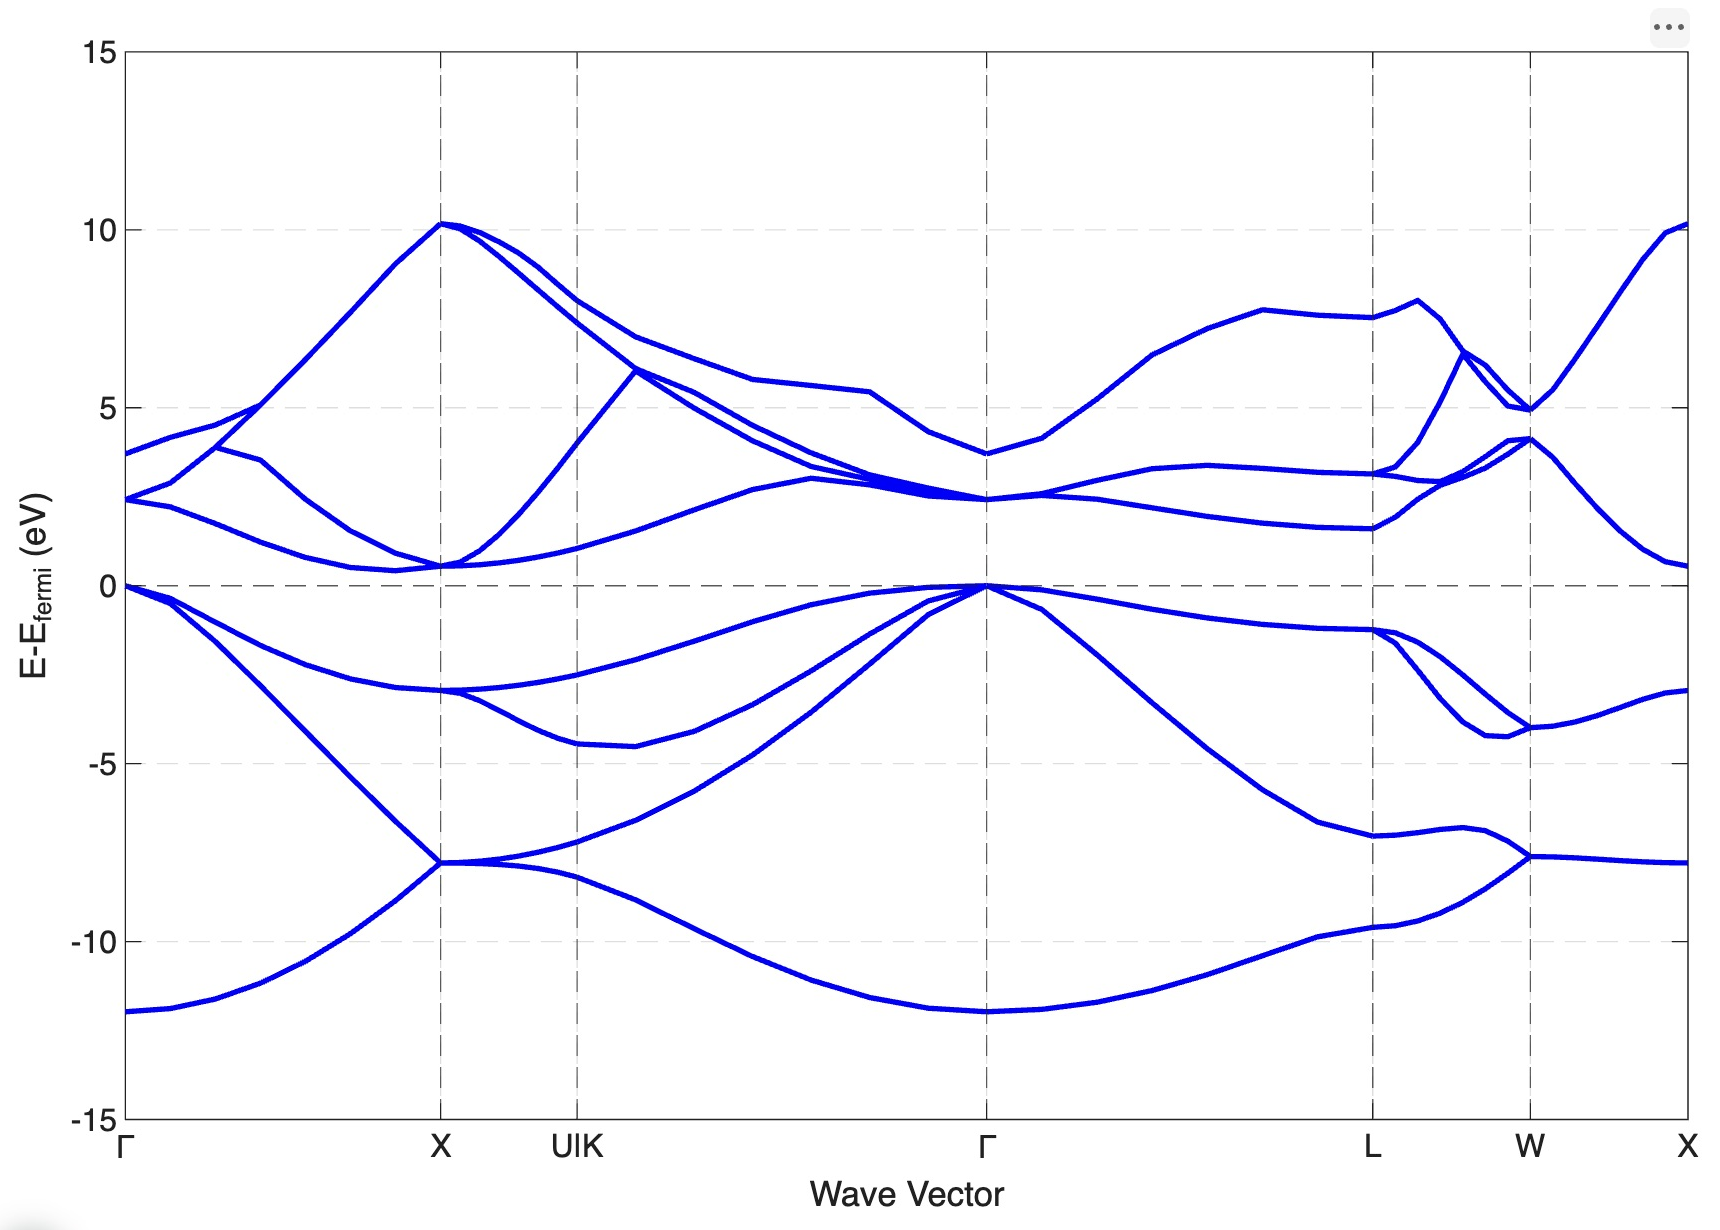
\includegraphics[width=\linewidth]{publication-assets/revision-silicon-bands-live.png}
\caption{硅两原子原胞能带在当前工具箱中的原生图形文档。使用随书保存数值重绘，整理字号及重复端点标签，未重新执行电子结构计算。}
\label{fig:si-bands-native}
\end{figure}

\subsection{先确认坐标和零点}

能带图横轴表示一条由若干高对称点组成的路径，纵轴表示能量。本书图中纵轴为 $E-E_{\mathrm{fermi}}$，单位 eV，因此零点是本次计算的费米能参考。不同路径段之间可能有分隔线或标签，不一定表示它们在倒空间中都连续相接。

曲线的横向位置由路径距离确定，并不是把三个 k 坐标中的某一个直接拿来作横轴。读图时可以先辨认路径标签，再观察费米能附近的占据态与未占据态，最后查看更深的价带或更高的空态。

图中每一条曲线表示一个能带分支，不是一个原子的运动轨迹。本例保存八条能带，所有曲线采用相同的蓝色；不能把线条颜色理解为元素、轨道或自旋分类。沿同一条曲线从左向右阅读，可以观察这条带随路径改变的能量；在同一横坐标处由下向上阅读，则是在比较该k点的不同能带。

高对称点之间的竖向虚线用于划分路径区段。若两段并不首尾相接，分界处可以出现组合标签；例如\ui{U|K}表示前一段到U结束、下一段从K开始，不是名为“U|K”的一个新k点。跨过这种分界时，不应把两侧曲线的接续当作沿同一方向连续行进。

\subsection{判断带隙}
\index{Daixi@带隙}

在通常的半导体描述中，较高的占据能带属于价带，较低的未占据能带属于导带。价带最高点与导带最低点之间的能量差称为带隙。若两者位于相同 k 点，通常称为直接带隙；位于不同 k 点，则称为间接带隙。

一条有限路径不一定经过真正的带边位置。即使图形很平滑，也不能仅凭路径上没有出现更低导带就断定它已经找到了全布里渊区的最小值。对于带隙研究，应结合更充分的采样和带边分析。

本书硅例主要用于熟悉能带工作流，采用较粗的入门网格。它展示了计算和绘图方法，未把目测带隙写成材料数据库中的标准值。整理计算报告时，先说明采用的条件，再讨论网格和泛函可能怎样影响结果。

\subsection{比较两张能带图}

比较之前，检查晶胞、路径、能量零点、泛函、赝势和带数是否一致。改变原胞与超胞可能导致能带折叠，图上曲线数量增加并不必然表示出现了新的物理态。改变零点也可能使整张图上下平移。

若研究形变的影响，可以保持同一套计算思路，对各个结构分别完成自洽，再使用可比较的路径。先观察变化主要发生在哪些能带和 k 点，再决定是否需要更精细的采样。把每一处微小位移都解释为新的物理效应之前，先排除数值条件不一致。

\section{阅读总态密度}
\index{Taimidu@态密度（DOS）}

\subsection{打开并核对总态密度图}

继续使用前一节已打开的\file{silicon-band-primitive.ks}。这份二原子原胞项目同时保存了一组$4\times4\times4$网格的总态密度数值，可以直接重绘，不必先关闭项目或运行新的DOS流程。

\begin{steps}
\item 确认当前仍为二原子原胞项目。在已经加入随书示例目录的MATLAB\regmark{}命令窗口执行：
\begin{lstlisting}[language=Matlab]
show_reference_results("dos");
\end{lstlisting}
\item 等待\ui{Density of States (DOS)}图形显示，并在\ui{Results → Plots}中核对新增条目。本图对应当前项目的Si2原胞，与另一份八原子晶胞项目区分。
\item 先看纵轴\ui{Energy (eV)}，再看横轴\ui{Density of States (DOS)}。曲线向右伸得越远，表示相应能量附近的总态密度越高；不能按普通“横轴能量”的习惯从左向右读取能区。
\item 沿纵轴找到零能量，再分别查看其下方、附近和上方的曲线。先描述有态区间、低态密度区间及主要峰，再考虑更细的小起伏。
\item 使用图形保存工具导出当前曲线，并保留含原始结果的项目。重新打开图片检查两个坐标轴都在画面中。
\end{steps}

这组DOS在$-10$至$10$ eV之间以$0.05$ eV步长取样，使用PBE、default赝势和20 Ha截断能。希望改变网格或能量范围时，按第\ref{ch:workflows}章导入\ui{DOS}模板，选择二原子原胞，填写新的参数并运行；重绘已有数组本身不会增加采样精度。




\begin{figure}[!htb]
\centering
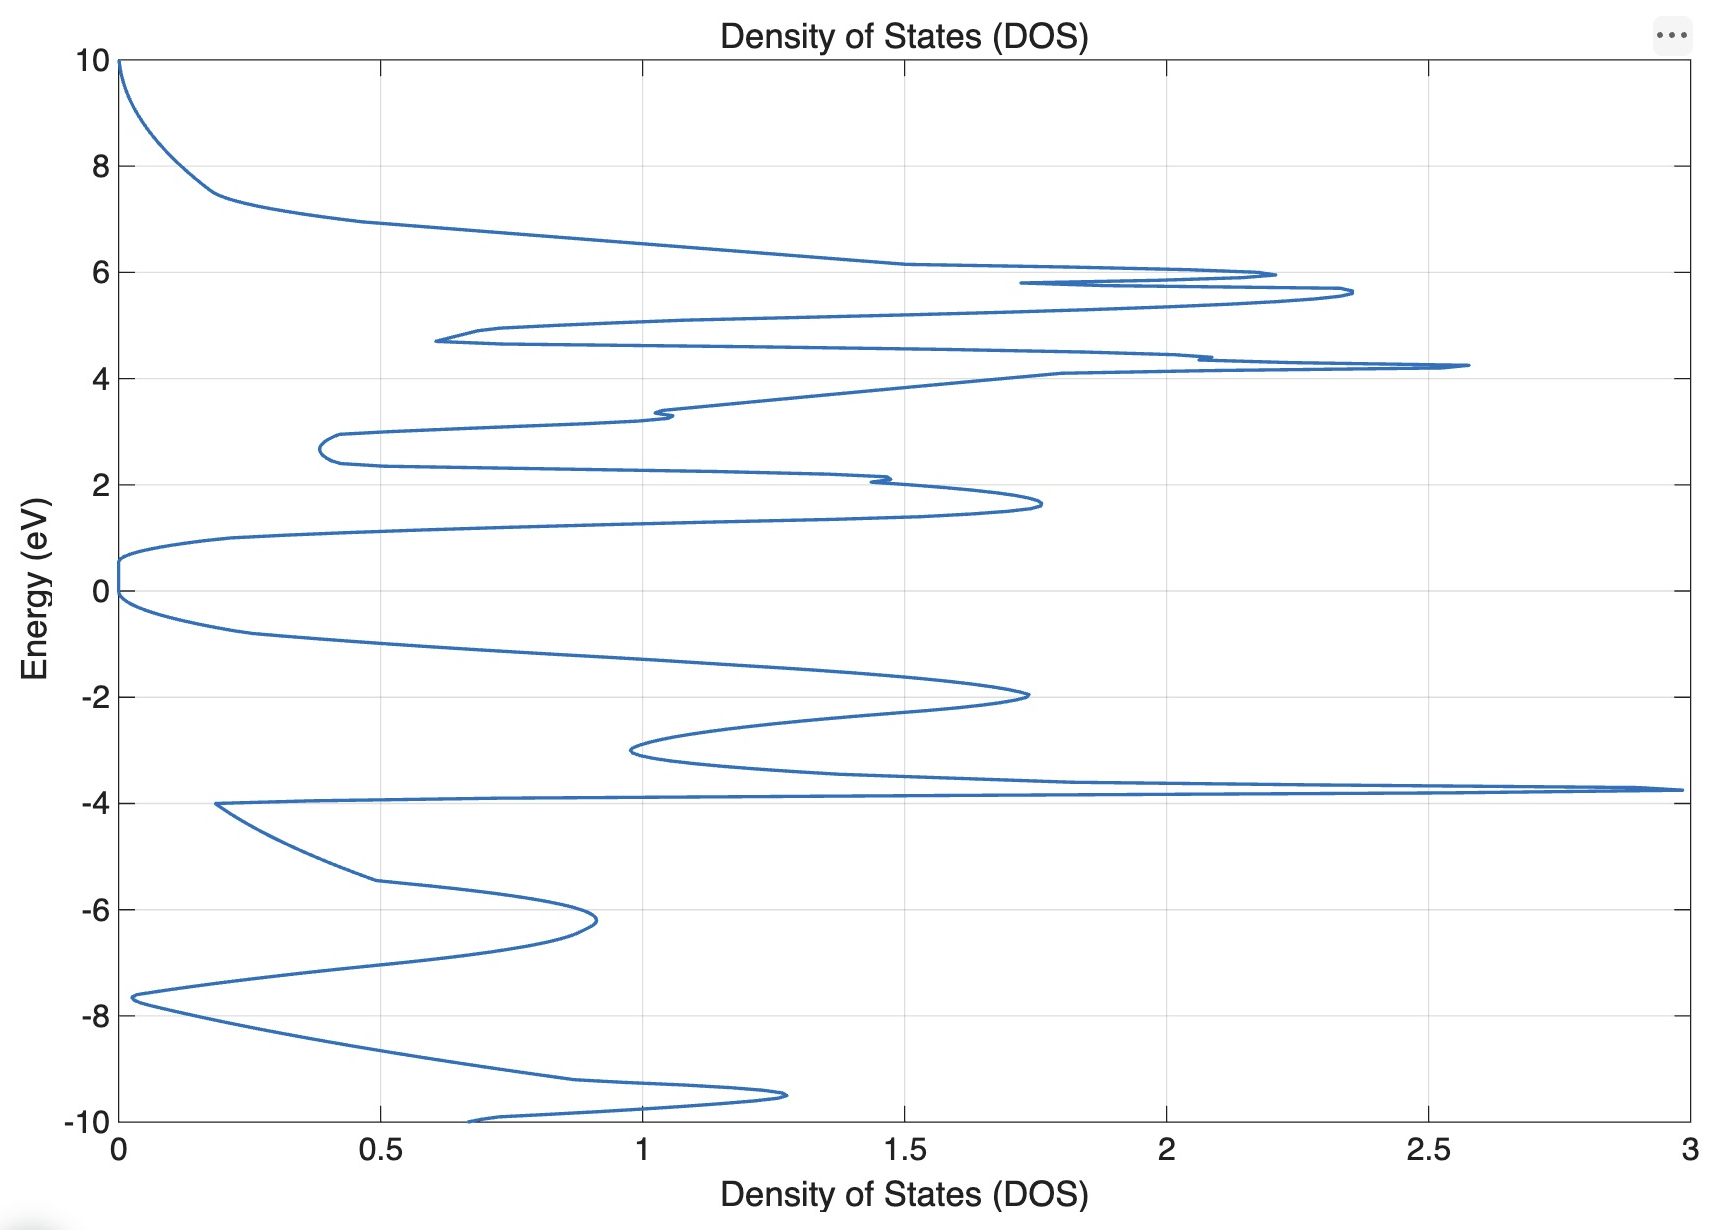
\includegraphics[width=\linewidth]{publication-assets/revision-silicon-dos-live.png}
\caption{同一硅两原子原胞的总态密度实机图，横轴为态密度、纵轴为能量。由随书保存的数值通过原生显示任务重绘。}
\label{fig:si-dos-native}
\end{figure}

\subsection{峰和低密度区域}

态密度在某个能量附近较高，表示这一能量范围聚集了较多电子态。曲线中的峰往往与能带的色散特征有关，但峰本身不直接告诉我们电子主要来自哪一种原子或轨道。那需要进一步的投影或成分分析。

本教程的 DOS 节点计算总态密度。不要把某个峰直接命名为“某元素的 p 轨道峰”，除非有相应的投影数据支持。对于元素单质，总态密度仍然汇集了不同轨道和不同 k 点的信息。

\subsection{与能带图联合阅读}

把能带和 DOS 放在相同能量参照下，可以先定位费米能，再观察哪些能区有较多电子态，哪些能区没有态。能带图展示沿路径的变化，DOS 则汇总整个网格的统计，两者从不同角度描述同一电子结构。

\file{silicon-tutorial.ks}另存八原子常规晶胞的DOS数值。打开那份项目再执行同一条\texttt{show\_reference\_results("dos")}命令，得到的是Si8结果。下文图\ref{fig:si-dos-results}保留这份八原子参考曲线，供阅读坐标与峰形；它与前述原胞重绘对应不同晶胞。比较两者时，先统一每晶胞或每原子的归一化方式，以及计算条件和能量参照。

\begin{figure}[!htb]
\centering
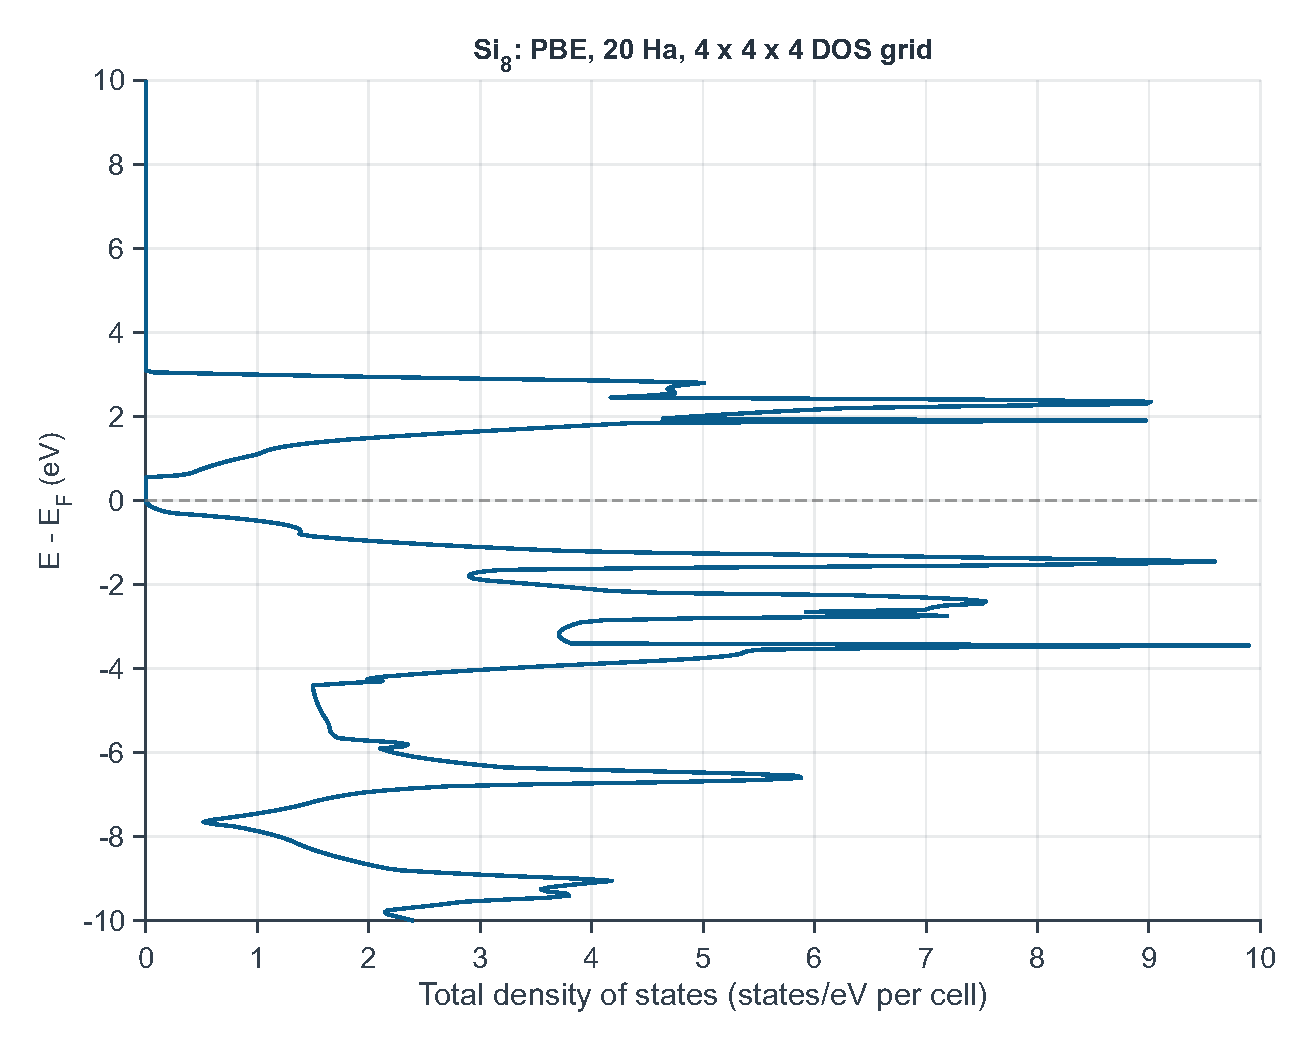
\includegraphics[width=\linewidth]{publication-assets/vector-02b7a0240bc7f99a0fc6.pdf}
\caption{八原子硅晶胞的参考总态密度。横轴为每晶胞、每电子伏特的态数，纵轴为相对费米能；本图采用入门练习的 $4\times4\times4$ 网格。}
\label{fig:si-dos-results}
\end{figure}

本软件的 DOS 图横轴为 DOS，纵轴为 Energy (eV)。若报告中把 DOS 放在能带图右侧，这种排列能够让两幅图共享由下到上的能量阅读方向。最终排版时，应保持两图的能量范围和零点一致。

\subsection{分辨采样细节与物理特征}

粗 k 点网格可能使 DOS 峰形变化明显，特别是在电子态较少或色散较强的能区。减小能量步长只能更密地评价当前近似曲线，不会增加布里渊区中的信息。判断某个小峰是否可靠，应比较更密网格下它是否仍然存在。

本书 $4\times4\times4$ 的硅 DOS 是入门起点。若把网格提高到 $8\times8\times8$，应比较主要峰位、费米附近低态密度区域和整体形状，而不是只看图线是否变得好看。不同精度下稳定保留的特征更值得继续分析。

\section{核对三维结果}

几何图适合展示原子位置、晶胞和局部环境。电子密度、势或轨道等空间数据则需要体数据查看器。导入实际的体数据文件后，可以使用等值面、切片和颜色映射观察它们的空间分布。

体数据的含义由输入文件和数据类型决定。一个标注为电子密度的 CUBE 文件与一个标注为轨道幅值的 CUBE 文件，虽然都能形成等值面，颜色和数值的物理解释却不同。先确认变量和单位，再选择等值面数值。

本书 SCF 工作流保存的计算结果不等于自动生成了所有常用体数据文件。若要展示某个空间量，应先取得相应数据，再按体数据章节的步骤导入。图注中注明变量、等值面值和单位，比只写“电子云”更清楚。

\section{整理原子结构视图}

本节使用原子结构文档自己的查看器。先打开随书硅结构，或打开已经检查过连接的分子，再从视图工具栏进入\ui{Viewer settings}。这里的设置用于观察和制图；工作流中的泛函、截断能和电子采样仍在计算节点中配置。

\subsection{记录位点与晶胞读数}

单击一个原子，在信息卡中核对位点序号和周期映像，再使用笛卡尔坐标或分数坐标旁的复制按钮，将数值粘贴到实验记录。复制保留的精度高于面板简写；笛卡尔坐标带\AA，分数坐标没有长度单位。记录周期映像时，同时写出\ui{Image}偏移，避免把相邻晶胞的显示位置当作输入位点的位置。

需要查看整张坐标表时，单击视图工具栏的\ui{Structure information}信息按钮，其提示为\ui{Fractional coordinates}。表中列出ID、元素、标签和五位小数的分数坐标，适合按位点查找；需要保留完整数值仍导出原生结构。分子没有周期分数坐标时，相应列显示横线。

晶体的胞长、夹角和体积可以从测量菜单的\ui{Cell parameters}读取。使用读数旁的复制按钮，将所需一组值粘贴到记录中，再补上结构文件名和当前晶胞表示。完成后关闭信息面板，继续取景；复制读数不会把模型另存为结构文件。

\subsection{比较晶胞表示和成键策略}

\ui{Scientific scene}集中管理场景分析。晶体的\ui{Change unit cell}可选\ui{Input cell}、\ui{Primitive cell}、\ui{Conventional cell}，以及Niggli和LLL两种约化晶胞。它们改变当前场景采用的晶胞表示；要把转换提交为项目中的模型，仍按建模章节使用原胞、惯用胞等结构命令。\ui{Repeat cell}则控制显示重复范围，不能代替构建计算超胞。

\begin{steps}
\item 打开硅结构的查看器设置，在\ui{Scientific scene}中保持\ui{Input cell}，记下当前位点数和晶胞。
\item 将\ui{Change unit cell}切换为\ui{Primitive cell}，等待场景重建完成。比较晶胞外框与位点排列，再切回\ui{Input cell}，确认回到原输入的表示。
\item 在\ui{Bonding strategy}中比较\ui{CrystalNN}与\ui{Minimum distance}，观察显示连接是否变化。一次只改一项，等待分析完成再读配位数或最近邻。
\item 将\ui{Repeat cell}的一个方向设为2，检查周期接续；完成后用\ui{Reset to 1 × 1 × 1}恢复。记录用于最终图片的表示、成键策略和重复范围。
\end{steps}

\begin{table}[htbp]
\centering\small
\caption{晶体查看器中的成键策略。}
\begin{tabularx}{\linewidth}{lX}
\toprule
选项 & 用途与读数的含义 \\
\midrule
CrystalNN & 按局部环境分析近邻，适合从完整配位环境开始观察。\\
Custom bonds & 使用VESTA截断规则；这里选择规则，不是在此输入任意键长。\\
Jmol bonding & 使用Jmol成键判据，便于与相应表示比较。\\
Minimum distance & 以最近距离及界面标出的10\%容差判断近邻。\\
O'Keeffe's algorithm & 按O'Keeffe判据识别近邻。\\
Hoppe's ECoN algorithm & 按有效配位分析识别近邻。\\
Brunner's reciprocal & 使用Brunner倒数距离判据。\\
\bottomrule
\end{tabularx}
\end{table}

分子的选项不同：\ui{Source topology · preferred}优先使用源连接，\ui{Source topology · explicit}明确使用源拓扑，\ui{OpenBabelNN · inferred}按几何推断。已有显式键的苯、吡啶或聚合物应先检查源连接，再决定是否比较推断结果。改变显示连接不会自动完成化学键编辑；需要改变分子拓扑时，使用添加键、删除键或设置键级。

\begin{figure}[H]
\centering
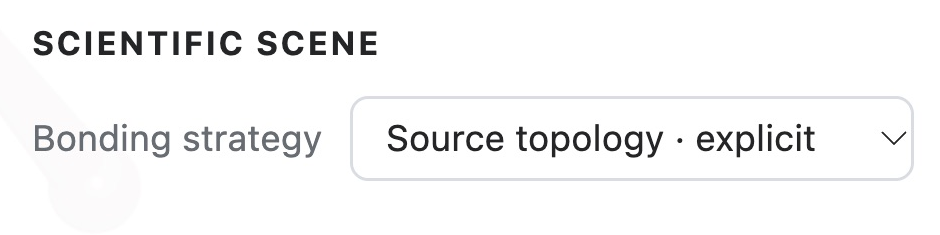
\includegraphics[width=90mm]{publication-assets/crop-1dadf5469e77f06dffe5.png}
\caption{中性单重态乙醇的\ui{Scientific scene}局部。该输入有9个原子、8条显式键，当前选择\ui{Source topology · explicit}，按原始连接显示分子。}
\label{fig:atomic-scientific-scene}
\end{figure}

\subsection{控制周期边界和辅助对象}

在\ui{Visibility}中先保留\ui{Atoms}、\ui{Bonds}和晶体的\ui{Unit cell}。\ui{Boundary image atoms}控制边界映像，\ui{One-hop bonded atoms}补充与当前显示原子直接相连的一层近邻，\ui{Hide incomplete bonds}隐藏缺少完整端点的连接。这几项会改变边界外观，应结合位点与映像编号阅读，不能只数画面中的球。

需要看局部配位时打开\ui{Polyhedra}；需要标明方向时保留\ui{Orientation axes}。\ui{Magnetic moments}用于显示数据中已有的磁矩，不会计算磁矩。分子另有\ui{Hydrogens}和\ui{Multiple bond order}，分别控制氢与多重键的显示。\ui{Continuous measurement}决定一次测量完成后是否继续选取下一组；连续测量不改变原子坐标。

在\ui{Style}中比较VESTA与Jmol元素配色，按图的用途选择\ui{Atomic}或\ui{Uniform}半径，再调整\ui{Atom scale}和\ui{Bond radius}。原子比例过大时可先减小球体，再判断是否有真正的短接触。\ui{Lighting \& surface}中的光照、材质、亮度和对比度用于改善辨识；需要回到起点时使用\ui{Reset appearance}。为一组比较图采用相同外观，并另外记录决定科学含义的结构和测量条件。

\section{导出原子结构视图}
\index{Yuanzi jiegou tuxiang@原子结构图像}

原子查看器的\ui{Export image}输出当前三维结构图，\ui{Export file}输出可交互页面、场景或结构文件。它们与体数据的等值面导出、工作流图形的保存工具分别工作。导出前先停止自动旋转、清除无关选择并确定取景。

\subsection{选择六种图像格式}

\begin{table}[H]
\centering\small
\caption{原子结构查看器的图像导出选项。}
\begin{tabularx}{\linewidth}{lX}
\toprule
菜单选项 & 适合的用途 \\
\midrule
PNG & 无损位图，适合技术文档与屏幕阅读。\\
JPEG & 压缩位图，便于分享；细线和文字应检查压缩效果。\\
TIFF & 无损位图，输出扩展名为\file{.tif}。\\
SVG & 矢量表达，适合继续排版或编辑线条。\\
PDF (Vector) & 矢量PDF，便于排版与放大阅读。\\
PDF (Raster) & 以栅格渲染保留当前场景的显示效果。\\
\bottomrule
\end{tabularx}
\end{table}

\begin{steps}
\item 打开需要的结构，调整视角和表示方式，确认晶胞、原子与必要标注都在画面内。
\item 在结构视图工具栏打开\ui{Export image}，先选PNG，填写保存位置；在线版完成浏览器下载。
\item 需要矢量版本时再导出SVG或\ui{PDF (Vector)}。矢量表达与栅格光照可能存在外观差别，应打开实际文件比较后选择。
\item 检查导出图的边界、文字和局部连接，把它与原始结构、项目及本次取景说明保存在同一练习目录。
\end{steps}

本菜单不使用后文计算结果图的72至600DPI设置。图像文件保存视图，不能据它重新取得完整的结构坐标；交换模型时还应导出结构文件。

% Native Online atomic-viewer menus; keep the original captures unchanged.
\begin{figure}[H]
\centering
\begin{minipage}[t]{58mm}
\vspace{0pt}
\centering
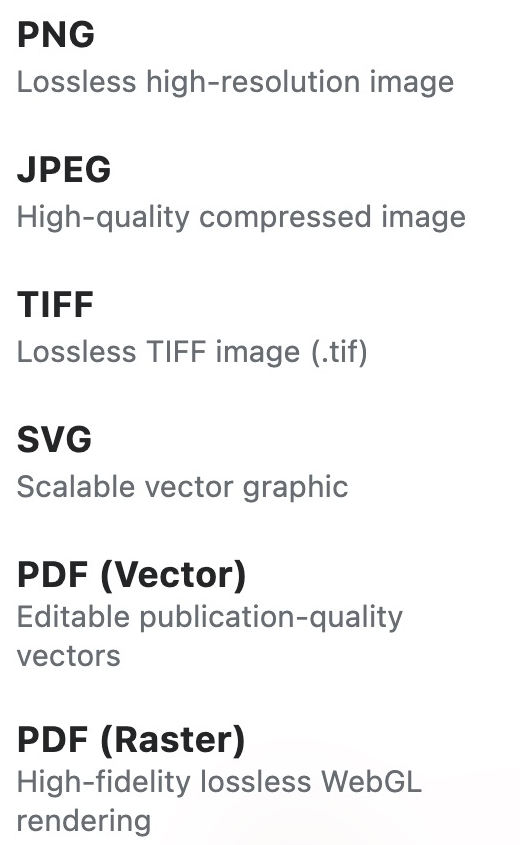
\includegraphics[width=52mm]{publication-assets/crop-496bc1fbfb3e99bfc4e7.png}
\end{minipage}\hspace{4mm}%
\begin{minipage}[t]{58mm}
\vspace{0pt}
{\centering
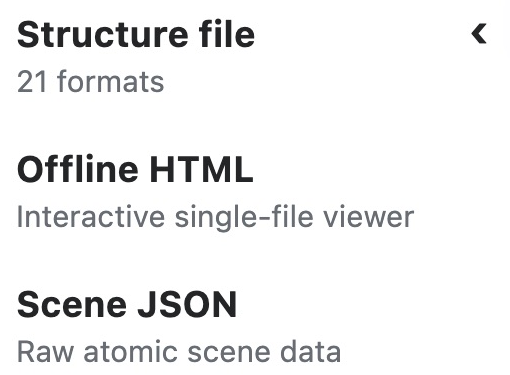
\includegraphics[width=51mm]{publication-assets/crop-68b4df9ea7d48ce9da1e.png}\par}
\par\vspace{3mm}
\raggedright\fontsize{9}{13}\selectfont
\ui{Structure file}保存所选格式能表达的模型信息。

\smallskip
\ui{Offline HTML}用于在本机浏览器中旋转观察。

\smallskip
\ui{Scene JSON}记录原子场景，区别于结构JSON。
\end{minipage}
\caption{原子查看器的两类导出菜单。左侧\ui{Export image}提供六种图像格式；右侧\ui{Export file}分别通向结构文件、离线页面与场景JSON。两幅菜单来自同一乙醇输入的不同显示状态。}
\label{fig:atomic-export-menus}
\end{figure}


\subsection{保存可以离线旋转的页面}
\index{Lixian HTML@离线 HTML}

\ui{Offline HTML}把当前原子场景、查看器外观设置与相机一起放入一个HTML文件，适合随计算报告提供可旋转的结构。它用于阅读场景，不能代替包含工作流、计算数据和编辑过程的项目。

\begin{steps}
\item 在原子结构视图中选好表示、重复范围和初始视角。
\item 打开\ui{Export file}，选择\ui{Offline HTML}，保存或下载生成的\file{-offline.html}文件。
\item 在本机浏览器中打开该文件，检查初始结构与外观，拖动旋转、滚轮缩放，并查看所需原子信息。
\item 分享时同时给出文件所表示的结构名称和用途；若还需继续建模或计算，再附原生结构与项目文件。
\end{steps}

离线页面保留导出时的场景。需要由工具箱重新分析成键、转换晶胞或继续提交模型时，回到原项目操作，再导出新的页面。

\subsection{区分场景\headinglatin{JSON}与结构\headinglatin{JSON}}

同一\ui{Export file}菜单中的\ui{Scene JSON}保存当前原子场景数据，可用于检查场景中的位点、显示映像、连接及分析说明。它没有把当前相机和全部外观设置一起写成查看器配置，也不是导出项目或计算输入的替代方式。

需要继续使用模型时，打开\ui{Structure file}子菜单，选原生JSON，保存后重新导入，核对晶格、位点、周期与属性。例如，扭转角、SQS搜索记录应从原生结构的\file{properties}读取；不要在名称带\file{-scene.json}的文件中寻找相同的模型记录。保存离线阅读版本则选\ui{Offline HTML}。三者都可保留，但应按用途命名，避免在另一台电脑上导入了错误文件。

随书的\file{ethanol-angle1095.json}是本节使用的中性单重态乙醇，包含9个原子、8条显式键，按1(C)—2(C)—3(O)定义的键角为$109.5^\circ$。\mbox{\file{ethanol-angle1095.png}}是同一模型通过PNG菜单导出的4032\,$\times$\,1964像素图像；\file{ethanol-angle1095-scene.json}则保存原子场景。继续编辑时导入结构JSON，后两份分别用于插图与检查场景记录。

\subsection{制作\headinglatin{Hero Shot}展示图}
\index{Hero Shot@Hero Shot}

Hero Shot提供另一种原子场景展示方式，适合突出整体形态和空间层次。它通过逐步细化渲染生成PNG，所用光照和材质不改变模型位置或电子结构结果。

\begin{steps}
\item 在结构查看器设置的\ui{Style → Theme}中选择\ui{Gleamoe Noir}。
\item 向下找到\ui{Hero Shot}，单击\ui{Enter Hero mode}。设置面板收起，进入专用取景界面。
\item 旋转、缩放结构，必要时用晶轴按钮确定方向。构图后保持视图稳定，让渐进渲染细化。
\item 打开\ui{Export Hero Shot}，先选\ui{High}。\ui{High}、\ui{Ultra}、\ui{Poster}分别标为视口的2.5、3和4倍导出比例。
\item 选择保存位置，等待渲染和写入结束。打开生成的\file{-hero.png}检查边界与细节；在线版还需确认浏览器下载完成。
\item 单击\ui{Exit Hero mode}返回普通查看器，继续测量或编辑；项目和原生模型仍按各自的保存步骤保留。
\end{steps}

首次练习用小模型与High设置，更容易比较取景和渲染效果。普通结构图适合清楚标注和几何比较；Hero Shot适合呈现形态，科学说明仍应给出模型来源、周期及必要的尺寸。

\section{导出计算结果图}

\subsection{选择适合用途的格式}

图形文档提供坐标轴工具，可以缩放、平移并导出图像。导出前先调整视图，确认标签完整、单位可见、线条没有被裁切。截图适合记录界面操作，正式报告中的数据图则通常更适合直接导出。

PNG 等位图格式适合放入文档和演示。PDF、SVG 等格式适合保留线条与文字的清晰度，但复杂图形或某些渲染内容可能采用不同输出方式。选择格式后，应打开实际文件检查一次，不能只根据扩展名判断质量。

在在线版中，导出文件通过浏览器下载。下载完成后，请到浏览器实际使用的下载位置检查文件；服务器端的会话路径不同于个人计算机上的保存位置。桌面版则根据文件对话框选择位置。

\subsection{在图形中查看细节}

把鼠标移到图形坐标区，按当前图形提供的工具进行平移、缩放、旋转或恢复视图。二维收敛图适合放大最后几步；布里渊区和能带曲面适合旋转。查看局部后先恢复整体范围，再导出需要完整呈现的结果，避免只保存一段被偶然放大的曲线。

三维能带曲面主要显示两张带边曲面。曲面之间的间隔不能未经坐标和采样检查就当作材料全局带隙；沿另一个方向可能还有更低的导带底或更高的价带顶。布里渊区图显示的是倒空间几何，也没有由多面体颜色编码出电子能量。新图形与原有路径能带、DOS分别承担不同问题，报告中应写明是哪一类图。

\subsection{在在线版中导出结果图}

在线版保留图形原生工具条，但保存和复制动作通过浏览器取得文件。选择保存图像后，会出现\ui{导出图片}窗口，可填写文件名、格式和分辨率。不要只把项目保存到云端，就认为已经把图片下载到了本机。

\begin{steps}
\item 打开需要的结果图，把坐标范围恢复到希望保存的状态。
\item 从图形工具条选择保存，填写有辨识度的文件名，例如\file{H2-SCF.png}。
\item 按用途选PNG、JPEG、TIFF、PDF或SVG。位图分辨率可在72至600DPI之间设置；屏幕阅读可先使用150DPI，打印用途再提高。
\item 单击\ui{保存}，随后完成浏览器的文件下载动作。
\item 从本机文件管理器打开实际下载文件，确认坐标轴、图例和图注需要的数值清楚完整。
\end{steps}

复制图像与复制矢量在浏览器环境中也会转为相应内容的文件取得流程；矢量动作提供SVG来源，不保证直接进入本机系统剪贴板。选择PDF或SVG时，DPI不能替代对字体、线条和实际输出效果的检查。保存图像也不会保存全部原始数组，所以还应保留项目和必要的数据文件。


\subsection{保存原始数值}
\index{Shuju daochu@数据导出}

项目文件保存运行数据，配套脚本还提供 MAT 或 CSV 结果，适合进一步计算和绘制统一样式的图。CSV 表格应有清楚的列含义，例如第一列为相对费米能的能量，第二列为 DOS。交换数据时，另附一行单位说明往往比依赖口头解释可靠。

需要拟合、积分或数值比较时，使用原始计算记录。截图适合展示趋势，读出的点会受到显示范围、分辨率和线宽影响。

\subsection{一幅可以独立阅读的图}

好的图注应让读者在不翻阅整个项目的情况下理解图形。结构图说明原子或晶胞，收敛图说明迭代量和单位，能带图说明路径与能量零点，DOS 图说明采样和能量参照。主要计算条件放在图注或附近正文即可，不需要把完整日志挤进图内。

为多张图使用一致的字体、字号、颜色和能量范围。不同图如果使用同一种颜色表示同一种量，读者便更容易比较。氢分子的初始与优化结构可以使用相同视角；两个 DOS 可以保持相同轴限；这些安排比增加装饰更能提高可读性。

\section{把结果写成一段完整说明}

一段清楚的结果说明通常依次交代问题、条件、观察和解释。例如，可以先说“在固定 $10$ Bohr 模拟盒中优化氢分子的键长”，随后给出 PBE、赝势和截断能，再报告键长缩短与能量降低，最后说明这些数值属于当前模型下的平衡结构。

避免只写“结果正常”或“符合预期”。更有用的表达是指出哪个量收敛、主要变化发生在哪里、比较时保持了哪些条件。若尚未完成某一项精度检查，可以清楚说明本次结果用于演示流程，并给出下一项有意义的检查，而不必用很长的笼统提醒淹没结果本身。

在关闭项目之前，保存当前工作，重新检查一次项目、输入文件和导出图形是否对应。一个能够打开、阅读和再次运行的项目，是这次计算最完整的记录。
